\documentclass{beamer}

\usetheme{metropolis}           % Use metropolis theme
\title{Funnel hopping Monte Carlo: An efficient method to overcome broken ergodicity}
\subtitle{Proseminar Computational Physics and Electronic Structure}
\date{\today}
\author{Matthias Vogler}
\institute{Departement of Physics\\ University of Basel}

\usepackage[backend=biber,style=ieee,natbib=true]{biblatex} % Use the bibtex backend with the authoryear citation style (which resembles APA)

\addbibresource{bibliography.bib} % The filename of the bibliography

\usepackage[autostyle=true]{csquotes} % Required to generate language-dependent quotes in the bibliography


\begin{document}
  \maketitle
  \section{Introduction}
  \begin{frame}
  \frametitle{The Paper}
   	\begin{itemize}
   		\item Funnel hopping Monte Carlo: An efficient mehtod to overcome broken ergodicity \cite{Finkler2020}
   		\item \citeauthor{Finkler2020} 
   		\item Journal of Chemical Physics
   		\item 23 April 2020

   	\end{itemize}
  \end{frame}

  \begin{frame}
  	\begin{center}
  		\huge
  		Monte Carlo Simulations and Metropolis-Hastings
  	\end{center}

  \end{frame}

  \begin{frame}
  	\frametitle{Monte Carlo simulations and Metropolis-Hastings}
  	\large Goal: Generate random samples from a target distribution \\
  	\subsubsection{Algoritm}
  	\begin{enumerate}
  		\item Start at initial configuration $\mathbf{r}$
  		\item Propose a new configuration $\mathbf{r}^\prime$
  		\item Accept or reject the new configuration with the probability $\alpha$ given by the Metropolis-Hastings criterion \cite{Hastings1970}
  		\begin{equation}
  		\alpha = \text{min}\left(1,\frac{P(\mathbf{r}^\prime)}{P(\mathbf{r})}\frac{g(\mathbf{r}|\mathbf{r}^\prime)}{g(\mathbf{r}^\prime|\mathbf{r})}\right)
  		\end{equation}
  	\end{enumerate}
  \end{frame}

  \begin{frame}
  	\frametitle{Monte Carlo simulations and Metropolis-Hastings}
  	\begin{itemize}
  		\item $P(\mathbf{r})$: target distribution
  		\item $g(\mathbf{r}^\prime|\mathbf{r})$: probability of proposing a move from $\mathbf{r}$ to $\mathbf{r}^\prime$
  		\item Our target distribution is the Boltzmann distribution:
  		\begin{equation}
  			P(r) = \frac{1}{Z(T)}\exp\left(\frac{-E(\mathbf{r})}{k_bT}\right)
  		\end{equation}
  		\item Note: $\mathbf{r} = (\vec{r}_1,\vec{r}_2, \ldots, \vec{r}_{N})^\text{T}$
  	\end{itemize}
  \end{frame}

  \begin{frame}
  \frametitle{Monte Carlo simulations and Metropolis-Hastings}
  	Proposing a new configuration $r'$ is done by small random atomic displacements but...
  	\begin{itemize}
 		\item Displacements should be sufficiently \emph{small} or the sampling will always reject the proposed configuration
   		\item Displacements should be sufficiently \emph{large} or the sampling will be inefficient
	\end{itemize}
	$\Longrightarrow$ Inherent trade-off between size of the moves and the resulting acceptance rate
  \end{frame}
	
	\begin{frame}
		\frametitle{Monte Carlo simulations and Metropolis-Hastings}
		We would like to sample the complete configuration space but this brings some problems in practice
		\begin{itemize}
			\item High energy barriers between different regions
			\item limited computation time
		\end{itemize}	
	\end{frame}

	\begin{frame}
		\frametitle{Energy Landscapes}
		\begin{itemize}
		\item Energy landscapes can best be characterized by its local minima.
		\item Very low local minima are usaly surrounded by higher lying local minima.
		\item These can be grouped into so-called \emph{funnels}
	\end{itemize}
	This is best visualized by disconnectivity graphs \cite{Wales2012}.
	\end{frame}

	\begin{frame}
		\frametitle{Energy Landscapes}
		\begin{figure}
			\center
			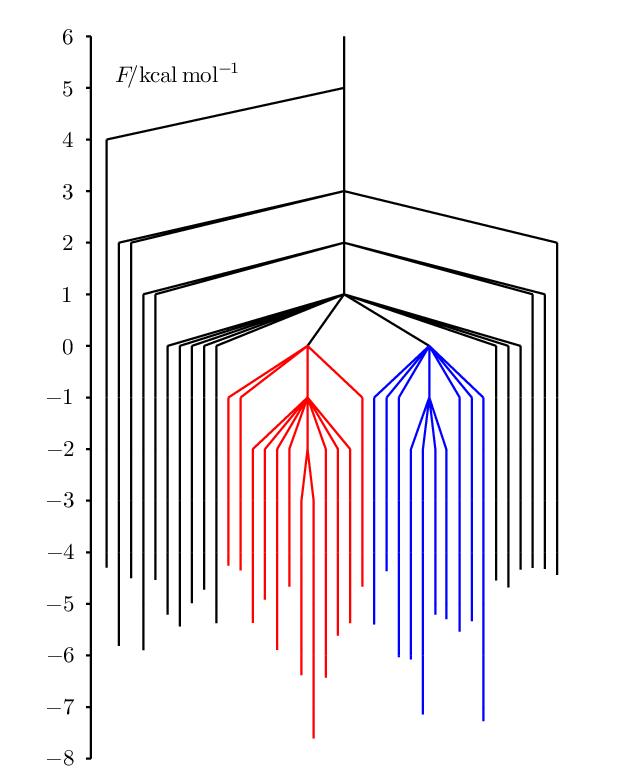
\includegraphics[height=0.75\textheight]{figures/funnels.png}
			\label{fig:funnels}
			\caption{Energy disconnectivity graph for met-enkephalin at 298 K. The low-energy region of the graph contains two funnels, highlighted in red and blue. Source: \cite{Wales2005}}
		\end{figure}
	\end{frame}

	\begin{frame}
		\frametitle{Broken Ergodicity}
		\begin{itemize}
			\item In systems with multiple Funnels, the energy barriers between these funnels can be very high
			\item Monte-Carlo simulations struggle to cross these barriers in the available simulation time
		\end{itemize}
		$\Longrightarrow$ Broken Ergodicity\\
		$\Longrightarrow$ The simulation does not reach every point in configuration space with non-zero probability
	\end{frame}

	\begin{frame}
		\frametitle{Current Methods example}
		\begin{itemize}
			\item Parallel Tempering (PT)
			\begin{itemize}
				\item Run at different $T$ in paralell and information is propagated down
				\item Low temperatures of interest necessitate many instances run in paralell $\Rightarrow$ inefficient
			\end{itemize}
		
		\end{itemize}
	\end{frame}

	\section{Funnel Hopping Monte Carlo:\\The Method}
	\begin{frame}
		\frametitle{Smart darting}
		\textbf{Idea:} Construct new MC moves using already known information about the local minima in the landscape
	\end{frame}

	\begin{frame}
		\frametitle{Smart darting}
		Given a set of $M$ local minima $\{\vec{R}_i\}_{i=1,2,\hdots,M}$ we define the \emph{darting vectors} $\vec{D}_{ij}$ as
		\begin{equation}
			\vec{D}_{ij}=\vec{R}_i-\vec{R}_j\quad | \quad i\neq j
		\end{equation}
		Furthermore, epsilon regions are placed arround each local minima to define if a configuration is inside such a minima region.\\
		If
		\begin{equation}
			||\vec{R}_i-\vec{r}_i||<\varepsilon
		\end{equation}
		then the configuration is considered inside the local minima.
	\end{frame}

	\begin{frame}
		\frametitle{Smart darting}
		The MCMC procedure is then amended by some \emph{darting moves}.\\
		New Procedure:
		\begin{enumerate}
			\item Draw a random number to decide if a darting move or a normal move is performed
			\item If a darting move is chosen, check if current configuration $\vec{r}$ is inside a epsilon region
			\begin{itemize}
				\item If false, reject the move
				\item If true, propose darting move
			\end{itemize}
			\item The configuration lies within the minimum $\vec{R}_i$ we randomly choose a darting vector starting at minimum $i$
			\item The new configuration is proposed by
			\begin{equation}
				\vec{r}'=\vec{r}+\vec{D}_{ij}
			\end{equation}
			\item Accept or reject the move with Metropolis criterion
		\end{enumerate}
	\end{frame}

	\begin{frame}
		\frametitle{Smart darting}
		Shortcomings:
		\begin{itemize}
			\item Minima of rotational and translational invariant systems aren't points in configuration space\\
			$\Rightarrow$ Minima is a hypersurface $\Rightarrow$ makes it impossible to define epsilon regions
			\item Real regions of low energies (and high probability) are often ellipsoidal and addition of darting vectors often miss the low energy regions around the local mimia
		\end{itemize}
	\end{frame}

	\begin{frame}
		\frametitle{Fixing rotation and translation}
		\begin{itemize}
			\item To implement a method that targets the desired regions with no assumption of their shape, one has to fix rotation and translation
			\item It is not trivial to identify equivalent configurations in $3N$ dimensional coodrinate space
		\end{itemize}
		$\Rightarrow$ But that's what the authors propose a method for and it gets very technical
	\end{frame}

	\begin{frame}
		\frametitle{RMSD and Eckart Space}
		To remove these degrees of freedom from our configurations, the paper assigns a special set of coordinates to the trans. and rot. invariant configuration $r$.
		\begin{itemize}
			\item Identify a reference configuration $R$ of a local minima
			\item Minimize the root mean squared deviation (RMSD) of $R$ to the configuration $r$
			\begin{equation}
				\text{RMSD}(r, R)=\sqrt{\frac{\sum_{i=1}^N ||\vec{r}_i-\vec{R}_i||^2}{N}}
			\end{equation}
		\end{itemize}
	\end{frame}

	\begin{frame}
		\frametitle{RMSD and Eckart Space}
		It was shown by \citeauthor{Kudin2005} \cite{Kudin2005} that the RMSD is minimal if the \emph{Eckart conditions} are met:
		\begin{equation}
			\sum_{i=1}^N \vec{r}_i - \vec{R}_i = \vec{0}
		\end{equation}
		\begin{equation}
			\sum_{i=1}^N \vec{r}_i \times \vec{R}_i = \vec{0}
		\end{equation}
	\end{frame}

	\begin{frame}
		\frametitle{RMSD and Eckart Space}
		Defining the displacement $d$ as
		\begin{equation}
			\vec{d}=\vec{r}_i-\vec{R}_i
		\end{equation}
		we can rewrite the Eckart conditions as
		\begin{equation}
			\sum_{i=1}^N \vec{d}_i= \vec{0}
			\label{eq:1}
		\end{equation}
		\begin{equation}
			\sum_{i=1}^N \vec{d}_i\times \vec{R}_i = \vec{0}
			\label{eq:2}
		\end{equation}

	\end{frame}		

	\begin{frame}
		\frametitle{RMSD and Eckart Space}
		The 6 linear equations contained in eq. \ref{eq:1} and eq. \ref{eq:2} are orthogonal to the six vectors
		\begin{equation}
		V^1=\begin{pmatrix} 1\\0\\0\\1\\0\\0\\1\\ \vdots\end{pmatrix},
		V^2=\begin{pmatrix} 0\\1\\0\\0\\1\\0\\0\\ \vdots\end{pmatrix},
		V^3=\begin{pmatrix} 0\\0\\1\\0\\0\\1\\0\\ \vdots\end{pmatrix},
		\end{equation}
	\end{frame}

	\begin{frame}
		\frametitle{RMSD and Eckart Space}
		\begin{equation}
			V^4=\begin{pmatrix}0 \\ \vec{R}_{1,z} \\ -\vec{R}_{1,y} \\ 0 \\ \vec{R}_{2,z} \\ -\vec{R}_{2,y} \\ 0 \\ \vdots \end{pmatrix},
			V^5=\begin{pmatrix}-\vec{R}_{1,z} \\ 0 \\ \vec{R}_{1,x} \\ -\vec{R}_{2,z} \\ 0 \\ \vec{R}_{2,x} \\ \vec{R}_{3,z} \\ \vdots\end{pmatrix},
			V^6=\begin{pmatrix}\vec{R}_{1,y}\\-\vec{R}_{1,x}\\0\\\vec{R}_{2,y}\\-\vec{R}_{2,x}\\0\\\vec{R}_{3,y}\\\vdots\end{pmatrix}
		\end{equation}
	\end{frame}

	\begin{frame}
		\frametitle{RMSD and Eckart Space}
		We can now construct $3N-6$ basis vectors $B^i$ that are orthonormal to $V^j$ and themselves:
		\begin{equation}
		||B^i||=1
		\end{equation}
		\begin{equation}
			B^i\cdot B^j = 0\quad\forall\quad i\neq j
		\end{equation}
		\begin{equation}
			B^i\cdot V^j = 0
		\end{equation}
	\end{frame}

	\begin{frame}
		\frametitle{RMSD and Eckart Space}
		\begin{itemize}
			\item Using $B^i$ as our basis, we can remove 6 degrees of freedom from the displacement vectors $d$
			\item This fixes the rotation and translation of the configuration
			\item Now we can assign a unique set of $3N-6$ coordinates to every configuration
		\end{itemize}
		$\Longrightarrow$ The 3N dimensional displacement vector $d$ is transformed to the $3N-6$ dimensional $d'$ with
		\begin{equation}
			d'_i=d\cdot B^i\quad|\quad i=1,2,\ldots, 3N-6
		\end{equation}
	\end{frame}

	\begin{frame}
		\frametitle{RMSD and Eckart Space}
		For systems with indistinguishable atoms, minimizing the RMSD also depends on the permutation.
		\begin{itemize}
			\item Optimal rotation depends on the permutation
			\item Optimal permutation depends on the rotation
		\end{itemize}
		$\Longrightarrow$ Causality dilemma
	\end{frame}

	\begin{frame}
		\frametitle{Minimizing the RMSD}
		\begin{itemize}
			\item For optimal rotation: Quaternion Algorithm \cite{Coutsias2004}
			\item For optimal permutation: Hungarian Algorithm \cite{Kuhn1955}
		\end{itemize}
		$\Longrightarrow$ Use both algorithms in alteration until a converged solution is found.
	\end{frame}

	\begin{frame}
		\frametitle{Funnel hopping Monte Carlo}
		The abbility to uniquely map structures to a $3N-6$ dimensional subspace is the foundation of FHMC.\\
		Now to the actual method:
		\begin{itemize}
			\item First we assign each point in config. space to its nearest minimum.
			\item For each minimum $R_i$ we assign a probability distribution $q_i(r)\in$ of the $3N-6$ dimensional space
		\end{itemize}	
		These $q_i(r)$ should cover the high probability regions around the associated mimimum.

		% Paper proposes to calculate over Gaussian mixtures. q_i(r) does not have to resemble boltzmann. q_i(r) allows for proposal of better moves -> efficient sampling
	\end{frame}

	\begin{frame}
		\frametitle{Funnel hopping Monte Carlo}
		To propose a funnel hopping move, we follow these steps:
		\begin{enumerate}
			\item Determine the minimum $R_i$ closest to current configuration
			\item Randomly choose one of the other minima $R_j$ and draw a configuration from the associated $q_j$
			\item The proposed move is then accepted with probability $\alpha$ over a modified Metropolis criterion:
				\begin{equation}
					{\scriptstyle
					\alpha(r\rightarrow r')=\text{min}\left(1,\exp\left(-\frac{E(r')-E(r)}{k_bT}\right)\frac{q_i(r)}{q_j(r')}\frac{T_{ji}}{T_{ij}}\frac{h_{\alpha i}}{h_{\alpha j}}\right)
					}
				\end{equation}
		\end{enumerate}
	\end{frame}

	\begin{frame}
		\frametitle{Funnel hopping Monte Carlo}
			$$
				\alpha(r\rightarrow r')=\text{min}\left(1,\exp\left(-\frac{E(r')-E(r)}{k_bT}\right)\frac{q_i(r)}{q_j(r')}\frac{T_{ji}}{T_{ij}}\frac{h_{\alpha i}}{h_{\alpha j}}\right)
			$$
			\begin{itemize}
				\item $T_{ij}$: Transistion matrix giving probability of choosing minimum $j$ when in mimnimum $i$
				\item $h_{\alpha i}$: Point group order of the $i$-th minimum
			\end{itemize}
	\end{frame}

	\begin{frame}
		\frametitle{Generating the distributions $q_i(r)$}
		Short recap on multivariate Gaussian distributions:
		\begin{equation}
			\mathcal{N}(\vec{x})=\frac{1}{(2\pi)^{D/2}|\Sigma|^{1/2}}\exp\left(-\frac{1}{2}(\vec{x}-\vec{\mu})^\text{T} \Sigma^{-1}(\vec{x}-\vec{\mu})\right)
		\end{equation}
		\begin{itemize}
			\item $\vec{\mu}$: mean vector
			\item $\Sigma$: covariance matrix
		\end{itemize}
	\end{frame}

	\begin{frame}
		\frametitle{Generating the distributions $q_i(r)$}
		The paper proposes to generate the distributions over \emph{Gaussian mixtures}.
		\begin{equation}
			q_i^{g.m.}(r)=\left.\sum_{k=1}^m a_i^k \mathcal{N}_i^k(r) \quad\right|\quad \sum_{k=1}^m a_i^k=1\text{ and } a_i^k \geq0\,\forall k
		\end{equation}
		\begin{itemize}
			\item $\mathcal{N}_i^k$: Gaussians with means $\mu_i^k$ and covariance $\Sigma_i^k$
			\item $a_k^i$: Weights
		\end{itemize}
		The  parameters $a_k^i$, $\mu_i^k$ and $\Sigma_i^k$ are determined by fitting the Gaussian mixture to samples form the Boltzmann distribution.
	\end{frame}


































\begin{frame}
  	\printbibliography[heading=bibintoc]

  \end{frame}
\end{document}